\chapter{8PSK \& Higher-Order PSK}
\label{ch:8psk}

\begin{nontechnical}
\textbf{8PSK is like using 8 different hand gestures instead of 4}---you can send 50\% more data per symbol, but the gestures are closer together, making them easier to confuse in noisy conditions.

\textbf{The progression:}
\begin{itemize}
\item \textbf{BPSK:} 2 positions (up/down) = 1 bit/symbol
\item \textbf{QPSK:} 4 positions (corners) = 2 bits/symbol
\item \textbf{8PSK:} 8 positions (compass directions) = 3 bits/symbol $\leftarrow$ \emph{We are here}
\item \textbf{16-PSK:} 16 positions = 4 bits/symbol
\item \textbf{32-PSK:} 32 positions = 5 bits/symbol
\end{itemize}

\textbf{The trade-off:} More positions means faster data rate (8PSK is 1.5$\times$ faster than QPSK), but positions are closer together. This makes them easier to confuse when noise is present, requiring stronger signals (higher SNR) to work reliably.

\textbf{Real-world use:} \textbf{DVB-S2} satellite broadcasting uses 8PSK for HD channels because satellite bandwidth is expensive. The 50\% data rate increase translates to 50\% more channels in the same bandwidth. The trade-off is needing larger receiving dishes for adequate SNR.

\textbf{Why not go higher?} Beyond 8PSK, phase states become too closely spaced. Even tiny noise causes errors. For higher spectral efficiency, \textbf{QAM} (which varies both amplitude and phase) is more effective. This is why WiFi uses 64-QAM and 256-QAM, not 16-PSK or 32-PSK.

\textbf{Where you'll encounter 8PSK:}
\begin{itemize}
\item Satellite TV (DVB-S2 HD channels)
\item Military SATCOM (MILSTAR)
\item NASA deep-space missions (high-rate data return)
\item Microwave backhaul (cell tower point-to-point links)
\end{itemize}

\textbf{Angular spacing matters:}
\begin{itemize}
\item QPSK: 90° between positions (robust)
\item 8PSK: 45° between positions (moderate)
\item 16-PSK: 22.5° between positions (sensitive)
\end{itemize}
Smaller angular separation = easier to confuse = requires cleaner signal and better phase tracking.
\end{nontechnical}

\section{Overview}

\textbf{8-ary Phase-Shift Keying (8PSK)} encodes data using \textbf{8 equally-spaced phase states} positioned around the unit circle, transmitting \textbf{3 bits per symbol}. This provides 50\% higher spectral efficiency than QPSK at the cost of approximately 3.5~dB additional SNR requirement.

\begin{keyconcept}
8PSK achieves \textbf{3 bits/symbol} ($\sim$2.2~bps/Hz with pulse shaping), providing a middle ground between QPSK's robustness (2 bits/symbol) and 16-QAM's efficiency (4 bits/symbol). Its constant envelope property makes it ideal for satellite systems using nonlinear power amplifiers.
\end{keyconcept}

Higher-order PSK schemes ($M$-PSK) use $M$ phase states to transmit $\log_2(M)$ bits per symbol. However, beyond 8PSK, the reduced angular spacing between constellation points makes phase noise and additive noise increasingly problematic, leading to rapid BER degradation.

\section{Mathematical Description}

\subsection{8PSK Constellation}

The 8PSK constellation consists of 8 equally-spaced phase states positioned on a unit circle with angular separation of $45°$ ($\pi/4$ radians):

\begin{equation}
\phi_m = \frac{2\pi m}{8} = \frac{\pi m}{4}, \quad m = 0, 1, \ldots, 7
\end{equation}
where:
\begin{itemize}
\item $\phi_m$ = phase angle for symbol $m$ (radians)
\item $m$ = symbol index from 0 to 7
\end{itemize}

\subsection{Time-Domain Signal}

The transmitted signal for symbol $m$ is:
\begin{equation}
s_m(t) = A\cos(2\pi f_c t + \phi_m)
\end{equation}
where:
\begin{itemize}
\item $A$ = carrier amplitude
\item $f_c$ = carrier frequency (Hz)
\item $\phi_m$ = phase for symbol $m$
\item $0 \leq t < T_s$ (symbol period)
\end{itemize}

\subsection{Complex Baseband Representation}

In complex baseband notation:
\begin{equation}
s_m = A e^{j\phi_m} = A e^{j\pi m/4}
\end{equation}

\textbf{IQ components:}
\begin{equation}
I_m = A\cos(\phi_m), \quad Q_m = A\sin(\phi_m)
\end{equation}
where:
\begin{itemize}
\item $I_m$ = in-phase component
\item $Q_m$ = quadrature component
\end{itemize}

\subsection{Constellation Diagram}

The 8PSK constellation places 8 symbols at equal angular spacing of $45°$ around the unit circle:

\begin{center}
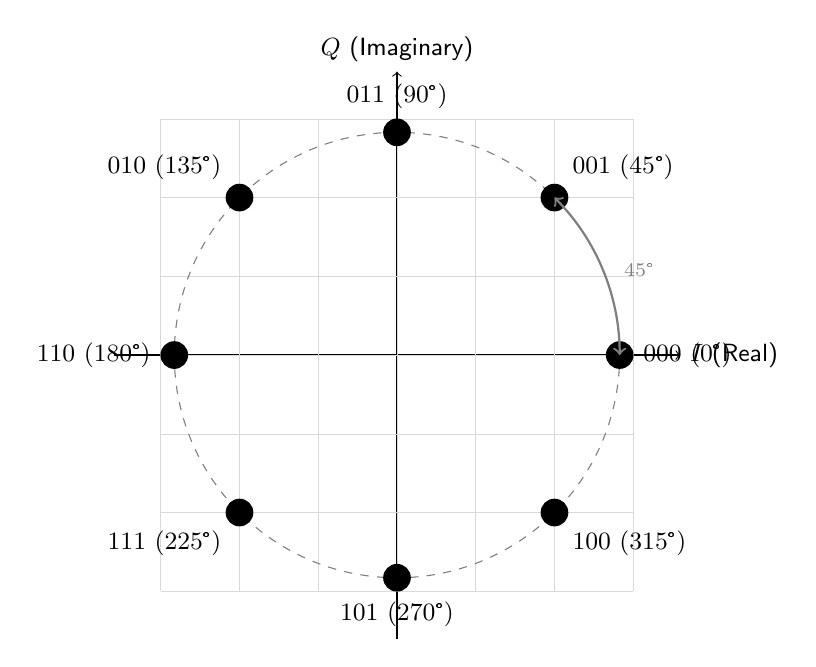
\begin{tikzpicture}[scale=2.0]
% Axes
\draw[->] (-1.8,0) -- (1.8,0) node[right] {\sffamily\small $I$ (Real)};
\draw[->] (0,-1.8) -- (0,1.8) node[above] {\sffamily\small $Q$ (Imaginary)};

% Grid
\draw[very thin,gray!30] (-1.5,-1.5) grid[step=0.5] (1.5,1.5);

% Unit circle
\draw[dashed,gray] (0,0) circle (1.4142);

% Constellation points with Gray coding
\fill[black] (1.4142,0) circle (2.5pt) node[right=5pt,font=\small] {000 (0°)};
\fill[black] (1,1) circle (2.5pt) node[above right=3pt,font=\small] {001 (45°)};
\fill[black] (0,1.4142) circle (2.5pt) node[above=5pt,font=\small] {011 (90°)};
\fill[black] (-1,1) circle (2.5pt) node[above left=3pt,font=\small] {010 (135°)};
\fill[black] (-1.4142,0) circle (2.5pt) node[left=5pt,font=\small] {110 (180°)};
\fill[black] (-1,-1) circle (2.5pt) node[below left=3pt,font=\small] {111 (225°)};
\fill[black] (0,-1.4142) circle (2.5pt) node[below=5pt,font=\small] {101 (270°)};
\fill[black] (1,-1) circle (2.5pt) node[below right=3pt,font=\small] {100 (315°)};

% Angular spacing annotation
\draw[<->,thick,gray] (1.4142,0) arc (0:45:1.4142) node[midway,right=4pt,font=\scriptsize] {45°};
\end{tikzpicture}
\end{center}

This maximum Euclidean distance constellation on the unit circle maintains constant envelope ($|s_m| = A$ for all $m$), enabling operation with nonlinear power amplifiers at saturation.

\subsection{Gray Coding}

Adjacent constellation points differ by only one bit (Gray coding) to minimize bit errors when symbol errors occur:

\begin{center}
\begin{tabularx}{\textwidth}{@{}ccXcc@{}}
\toprule
Symbol & Gray Code & Phase & $I_m/A$ & $Q_m/A$ \\
\midrule
0 & 000 & $0°$ & 1.000 & 0.000 \\
1 & 001 & $45°$ & 0.707 & 0.707 \\
2 & 011 & $90°$ & 0.000 & 1.000 \\
3 & 010 & $135°$ & $-0.707$ & 0.707 \\
4 & 110 & $180°$ & $-1.000$ & 0.000 \\
5 & 111 & $225°$ & $-0.707$ & $-0.707$ \\
6 & 101 & $270°$ & 0.000 & $-1.000$ \\
7 & 100 & $315°$ & 0.707 & $-0.707$ \\
\bottomrule
\end{tabularx}
\end{center}

Note that adjacent symbols (e.g., 000 $\rightarrow$ 001 $\rightarrow$ 011) differ by exactly one bit, minimizing the number of bit errors when noise causes a decision error to an adjacent symbol.

\section{Signal Characteristics}

\subsection{Constant Envelope Property}

All 8PSK symbols have identical amplitude:
\begin{equation}
|s_m| = A \quad \text{for all } m = 0, 1, \ldots, 7
\end{equation}

This constant envelope property provides a critical advantage:
\begin{itemize}
\item[\checkmark] Power amplifier can operate at saturation (maximum DC-to-RF efficiency)
\item[\checkmark] No amplitude modulation $\rightarrow$ no AM-PM distortion
\item[\checkmark] Peak-to-Average Power Ratio (PAPR) = 0~dB
\item[\checkmark] Compatible with nonlinear satellite TWTAs
\end{itemize}

\subsection{Symbol and Bit Energy}

The energy per symbol (normalized to unit symbol period $T_s = 1$):
\begin{equation}
E_s = \int_0^{T_s} |s_m(t)|^2 \, dt = A^2 T_s = A^2
\end{equation}

Since 8PSK transmits 3 bits per symbol:
\begin{equation}
E_b = \frac{E_s}{\log_2(8)} = \frac{E_s}{3} = \frac{A^2}{3}
\end{equation}
where:
\begin{itemize}
\item $E_s$ = energy per symbol (joules)
\item $E_b$ = energy per bit (joules)
\end{itemize}

\subsection{Minimum Euclidean Distance}

The minimum distance between adjacent constellation points is critical for noise immunity:
\begin{equation}
d_{\min} = 2A\sin\left(\frac{\pi}{8}\right) = 2A \times 0.3827 = 0.765A
\end{equation}

For normalized amplitude ($A = 1$): $d_{\min} = 0.765$

\textbf{Comparison with QPSK:}
\begin{itemize}
\item QPSK: $d_{\min} = \sqrt{2}A = 1.414A$ (at same average energy)
\item 8PSK: $d_{\min} = 0.765A$
\item \textbf{Ratio:} 8PSK minimum distance is $1.414/0.765 = 1.85\times$ smaller (5.3~dB)
\end{itemize}

This reduced separation explains why 8PSK requires approximately 3.5~dB higher SNR than QPSK to achieve the same BER.

\section{Modulation and Demodulation}

\subsection{Transmitter (IQ Modulator)}

The 8PSK modulator generates I and Q baseband components, then mixes with carrier quadrature signals:

\begin{center}
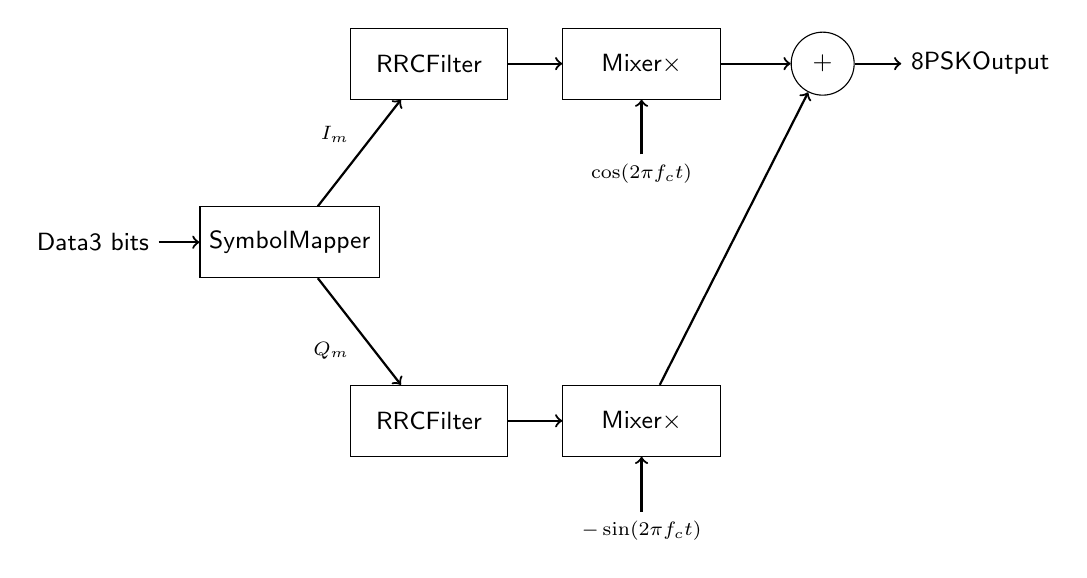
\begin{tikzpicture}[
  block/.style={rectangle, draw, minimum width=2cm, minimum height=0.9cm, font=\sffamily\small},
  node distance=2cm,
  font=\small
]
\node (input) {\sffamily Data\\3~bits};
\node[block, right of=input, node distance=2.5cm] (mapper) {Symbol\\Mapper};
\node[block, above right of=mapper, node distance=2.5cm, yshift=0.5cm] (i_filter) {RRC\\Filter};
\node[block, below right of=mapper, node distance=2.5cm, yshift=-0.5cm] (q_filter) {RRC\\Filter};
\node[block, right of=i_filter, node distance=2.7cm] (i_mult) {Mixer\\$\times$};
\node[block, right of=q_filter, node distance=2.7cm] (q_mult) {Mixer\\$\times$};
\node[circle, draw, right of=i_mult, node distance=2.3cm, minimum size=0.8cm] (sum) {$+$};
\node[right of=sum, node distance=2cm] (output) {\sffamily 8PSK\\Output};

\node[below of=i_mult, node distance=1.4cm, font=\scriptsize] (cos) {$\cos(2\pi f_c t)$};
\node[below of=q_mult, node distance=1.4cm, font=\scriptsize] (sin) {$-\sin(2\pi f_c t)$};

\draw[->,thick] (input) -- (mapper);
\draw[->,thick] (mapper) -- node[above left,font=\scriptsize] {$I_m$} (i_filter);
\draw[->,thick] (mapper) -- node[below left,font=\scriptsize] {$Q_m$} (q_filter);
\draw[->,thick] (i_filter) -- (i_mult);
\draw[->,thick] (q_filter) -- (q_mult);
\draw[->,thick] (cos) -- (i_mult);
\draw[->,thick] (sin) -- (q_mult);
\draw[->,thick] (i_mult) -- (sum);
\draw[->,thick] (q_mult) -- (sum);
\draw[->,thick] (sum) -- (output);
\end{tikzpicture}
\end{center}

\textbf{Process:}
\begin{enumerate}
\item \textbf{Symbol mapping:} Map 3-bit groups to I/Q coordinates using Gray coding
\item \textbf{Pulse shaping:} Apply root raised-cosine (RRC) filter to limit bandwidth
\item \textbf{Upconversion:} Mix I with $\cos(2\pi f_c t)$ and Q with $-\sin(2\pi f_c t)$
\item \textbf{Combine:} Sum I and Q paths to generate RF signal
\end{enumerate}

The transmitted signal is:
\begin{equation}
s_{\text{RF}}(t) = I_m(t) \cos(2\pi f_c t) - Q_m(t) \sin(2\pi f_c t)
\end{equation}
where $I_m(t)$ and $Q_m(t)$ are the pulse-shaped baseband waveforms.

\subsection{Receiver (Coherent Detector)}

\begin{center}
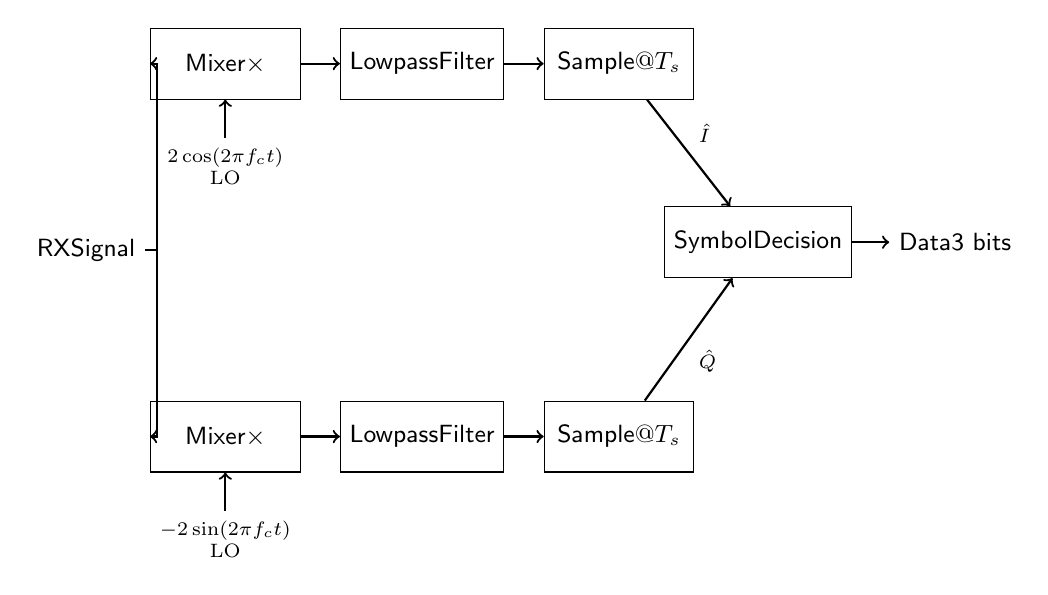
\begin{tikzpicture}[
  block/.style={rectangle, draw, minimum width=1.9cm, minimum height=0.9cm, font=\sffamily\small},
  node distance=1.9cm,
  font=\small
]
\node (input) {\sffamily RX\\Signal};
\node[block, above right of=input, node distance=2.5cm, yshift=0.6cm] (i_mult) {Mixer\\$\times$};
\node[block, below right of=input, node distance=2.5cm, yshift=-0.6cm] (q_mult) {Mixer\\$\times$};
\node[block, right of=i_mult, node distance=2.5cm] (i_lpf) {Lowpass\\Filter};
\node[block, right of=q_mult, node distance=2.5cm] (q_lpf) {Lowpass\\Filter};
\node[block, right of=i_lpf, node distance=2.5cm] (i_sample) {Sample\\$@T_s$};
\node[block, right of=q_lpf, node distance=2.5cm] (q_sample) {Sample\\$@T_s$};
\node[block, below right of=i_sample, node distance=2.5cm, yshift=-0.5cm] (decision) {Symbol\\Decision};
\node[right of=decision, node distance=2.5cm] (output) {\sffamily Data\\3~bits};

\node[below of=i_mult, node distance=1.3cm, font=\scriptsize, align=center] (lo_i) {$2\cos(2\pi f_c t)$\\LO};
\node[below of=q_mult, node distance=1.3cm, font=\scriptsize, align=center] (lo_q) {$-2\sin(2\pi f_c t)$\\LO};

\draw[->,thick] (input) -- ++(0.9,0) |- (i_mult);
\draw[->,thick] (input) -- ++(0.9,0) |- (q_mult);
\draw[->,thick] (lo_i) -- (i_mult);
\draw[->,thick] (lo_q) -- (q_mult);
\draw[->,thick] (i_mult) -- (i_lpf);
\draw[->,thick] (q_mult) -- (q_lpf);
\draw[->,thick] (i_lpf) -- (i_sample);
\draw[->,thick] (q_lpf) -- (q_sample);
\draw[->,thick] (i_sample) -- node[above right,font=\scriptsize] {$\hat{I}$} (decision);
\draw[->,thick] (q_sample) -- node[below right,font=\scriptsize] {$\hat{Q}$} (decision);
\draw[->,thick] (decision) -- (output);
\end{tikzpicture}
\end{center}

\begin{warningbox}
\textbf{Phase synchronization is critical.} The local oscillator must be exactly in phase with the transmitter carrier. A phase offset $\phi_e$ rotates the entire constellation, degrading performance. At $\phi_e = 22.5°$ (midpoint between symbols), complete decision ambiguity occurs.
\end{warningbox}

\textbf{Detection process:}
\begin{enumerate}
\item \textbf{Downconvert:} Mix received signal with local I/Q carriers
\item \textbf{Lowpass filter:} Remove $2f_c$ component, retain baseband
\item \textbf{Sample:} Capture I and Q values at optimal sampling instant
\item \textbf{Decision:} Find closest of 8 constellation points
\end{enumerate}

\textbf{Decision rule:} Calculate phase angle and quantize:
\begin{equation}
\hat{\phi} = \arctan\left(\frac{\hat{Q}}{\hat{I}}\right)
\end{equation}
\begin{equation}
\hat{m} = \left\lfloor \frac{\hat{\phi} + \pi/8}{2\pi/8} \right\rfloor \bmod 8
\end{equation}

The decision regions are 8 pie-slice wedges, each spanning $45°$ ($\pi/4$ radians), centered on each constellation point.

\subsection{Differential 8PSK (D8PSK)}

Differential encoding avoids the carrier phase ambiguity inherent in coherent PSK systems.

\textbf{Encoding:} Data is encoded in the \emph{phase change} between consecutive symbols:
\begin{equation}
\phi_k = \phi_{k-1} + \Delta\phi_k \bmod 2\pi
\end{equation}
where $\Delta\phi_k \in \{0, \pi/4, \pi/2, 3\pi/4, \pi, 5\pi/4, 3\pi/2, 7\pi/4\}$ encodes 3 data bits.

\textbf{Demodulation:} Compute phase difference between consecutive received symbols:
\begin{equation}
\Delta\hat{\phi}_k = \hat{\phi}_k - \hat{\phi}_{k-1}
\end{equation}

The 3-bit data word is decoded from $\Delta\hat{\phi}_k$ rather than from the absolute phase $\hat{\phi}_k$.

\textbf{Trade-off:}
\begin{itemize}
\item[\checkmark] No carrier phase recovery needed (only frequency synchronization)
\item[\checkmark] Simpler receiver implementation
\item[\checkmark] Immune to 8-fold phase ambiguity
\item[\texttimes] Approximately 3~dB performance penalty versus coherent detection
\item[\texttimes] Error propagation (one symbol error affects two decoded symbols)
\end{itemize}

\section{Bit Error Rate (BER) Performance}

\subsection{Symbol Error Rate in AWGN}

For 8PSK in additive white Gaussian noise (AWGN) with coherent detection (high SNR approximation):
\begin{equation}
P_s \approx 2Q\left(\sqrt{\frac{2E_s}{N_0}} \sin\left(\frac{\pi}{8}\right)\right) = 2Q\left(0.765\sqrt{\frac{E_s}{N_0}}\right)
\end{equation}
where:
\begin{itemize}
\item $P_s$ = symbol error probability
\item $E_s$ = energy per symbol (joules)
\item $N_0$ = noise power spectral density (W/Hz)
\item $Q(x) = \frac{1}{\sqrt{2\pi}} \int_x^\infty e^{-t^2/2} \, dt$ (Gaussian Q-function)
\end{itemize}

\subsection{Bit Error Rate with Gray Coding}

With Gray coding, most symbol errors cause only a single bit error:
\begin{equation}
\mathrm{BER} \approx \frac{P_s}{\log_2(8)} = \frac{P_s}{3}
\end{equation}

Expressing BER in terms of $E_b/N_0$ using $E_s = 3E_b$:
\begin{equation}
\mathrm{BER} \approx \frac{2}{3}Q\left(0.765\sqrt{\frac{3E_b}{N_0}}\right) = \frac{2}{3}Q\left(1.325\sqrt{\frac{E_b}{N_0}}\right)
\end{equation}

\subsection{Required $E_b/N_0$ for Target BER}

To achieve BER $= 10^{-6}$:

\begin{center}
\begin{tabular}{@{}lcc@{}}
\toprule
Modulation & Required $E_b/N_0$ (dB) & Penalty vs BPSK \\
\midrule
BPSK & 10.5 & --- \\
QPSK & 10.5 & 0~dB \\
\textbf{8PSK} & \textbf{14.0} & \textbf{+3.5~dB} \\
16-PSK & 18.0 & +7.5~dB \\
32-PSK & 22.0 & +11.5~dB \\
\bottomrule
\end{tabular}
\end{center}

\textbf{Key observation:} Each doubling of $M$ (from $M$-PSK to $2M$-PSK) adds approximately 3.5--4~dB SNR requirement, making higher-order PSK increasingly impractical.

\subsection{BER Performance Comparison}

\begin{center}
\begin{tabularx}{\textwidth}{@{}Xcccc@{}}
\toprule
$E_b/N_0$ (dB) & BPSK & QPSK & 8PSK & 16-PSK \\
\midrule
6 & $1.9 \times 10^{-3}$ & $1.9 \times 10^{-3}$ & $4.0 \times 10^{-2}$ & $1.5 \times 10^{-1}$ \\
8 & $5.6 \times 10^{-5}$ & $5.6 \times 10^{-5}$ & $8.0 \times 10^{-3}$ & $8.0 \times 10^{-2}$ \\
10 & $3.9 \times 10^{-6}$ & $3.9 \times 10^{-6}$ & $7.0 \times 10^{-4}$ & $3.0 \times 10^{-2}$ \\
12 & $7.8 \times 10^{-8}$ & $7.8 \times 10^{-8}$ & $4.0 \times 10^{-5}$ & $8.0 \times 10^{-3}$ \\
14 & $7.7 \times 10^{-10}$ & $7.7 \times 10^{-10}$ & $1.0 \times 10^{-6}$ & $7.0 \times 10^{-4}$ \\
\bottomrule
\end{tabularx}
\end{center}

\textbf{Key observation:} At a given SNR, higher-order PSK schemes suffer significantly higher BER due to reduced minimum distance between constellation points. To maintain the same BER as lower-order schemes, higher SNR is required.

\section{Bandwidth Efficiency}

The symbol rate for $M$-ary modulation is:
\begin{equation}
R_s = \frac{R_b}{\log_2(M)} \quad \text{(symbols/second)}
\end{equation}
where $R_b$ is the bit rate (bps).

With raised-cosine pulse shaping (roll-off factor $\alpha$), the occupied bandwidth is:
\begin{equation}
B = (1 + \alpha) R_s = (1 + \alpha) \frac{R_b}{\log_2(M)} \quad \text{(Hz)}
\end{equation}

The spectral efficiency (data rate per unit bandwidth) is:
\begin{equation}
\eta = \frac{R_b}{B} = \frac{\log_2(M)}{1 + \alpha} \quad \text{(bps/Hz)}
\end{equation}

\subsection{Comparison of PSK Schemes}

For $\alpha = 0.35$ (typical raised-cosine roll-off):

\begin{center}
\begin{tabularx}{\textwidth}{@{}lccXX@{}}
\toprule
Modulation & Bits/Symbol & $\eta$ (bps/Hz) & Required $E_b/N_0$ & Relative SNR \\
\midrule
BPSK & 1 & 0.74 & 10.5~dB & Baseline \\
QPSK & 2 & 1.48 & 10.5~dB & 0~dB \\
\textbf{8PSK} & \textbf{3} & \textbf{2.22} & \textbf{14.0~dB} & \textbf{+3.5~dB} \\
16-PSK & 4 & 2.96 & 18.0~dB & +7.5~dB \\
32-PSK & 5 & 3.70 & 22.0~dB & +11.5~dB \\
\bottomrule
\end{tabularx}
\end{center}

\begin{calloutbox}{Efficiency Trade-off}
8PSK provides 50\% higher spectral efficiency than QPSK (2.22 vs 1.48~bps/Hz) but requires 3.5~dB more SNR to achieve the same BER. This makes 8PSK ideal for bandwidth-limited systems with adequate link margin, such as:
\begin{itemize}
\item Satellite broadcasting (DVB-S2)
\item Microwave backhaul links
\item High-throughput military SATCOM
\end{itemize}
\end{calloutbox}

\section{Higher-Order PSK}

\subsection{16-PSK}

16-PSK extends the concept to 16 phase states with $22.5°$ angular spacing:
\begin{itemize}
\item \textbf{Phase states:} 16 ($M = 16$)
\item \textbf{Bits per symbol:} 4
\item \textbf{Angular spacing:} $22.5° = \pi/8$ radians
\item \textbf{Spectral efficiency:} $\sim$2.96~bps/Hz ($\alpha = 0.35$)
\end{itemize}

\textbf{Minimum distance:}
\begin{equation}
d_{\min} = 2A\sin\left(\frac{\pi}{16}\right) = 2A \times 0.1951 = 0.39A
\end{equation}

This is only half the minimum distance of 8PSK ($d_{\min} = 0.765A$), explaining the $\sim$4~dB performance penalty. The tight angular spacing makes 16-PSK extremely sensitive to:
\begin{itemize}
\item Phase noise from local oscillators
\item Frequency offset and drift
\item Timing jitter
\item Multipath fading
\end{itemize}

\textbf{Practical consideration:} 16-PSK is rarely used because 16-QAM provides similar spectral efficiency with better BER performance.

\subsection{32-PSK and Beyond}

\textbf{32-PSK:} $11.25°$ spacing, 5 bits/symbol

\textbf{64-PSK:} $5.625°$ spacing, 6 bits/symbol

\begin{warningbox}
PSK schemes beyond 8PSK ($M > 8$) are rarely used in practice. The extremely small angular spacing makes them highly sensitive to phase noise, frequency offset, and channel impairments. \textbf{QAM modulation} (which varies both amplitude and phase) provides superior performance for $M > 8$.
\end{warningbox}

\textbf{Why QAM wins for $M > 8$:}
\begin{itemize}
\item Larger minimum distance for same average power
\item Better noise immunity
\item Comparable implementation complexity
\item Industry standard (WiFi, LTE, cable modems use 16/64/256-QAM, not 16/64/256-PSK)
\end{itemize}

\section{Comparisons and Trade-offs}

\subsection{8PSK vs 16-QAM}

At similar spectral efficiency ($\sim$2.2~bps/Hz):

\begin{center}
\begin{tabular}{@{}lcc@{}}
\toprule
Parameter & 8PSK & 16-QAM \\
\midrule
Bits/symbol & 3 & 4 \\
Spectral efficiency & 2.22~bps/Hz & 2.96~bps/Hz \\
Required $E_b/N_0$ (BER $10^{-6}$) & 14.0~dB & 14.5~dB \\
Envelope & Constant (PAPR = 0~dB) & Variable (PAPR $\sim$2.6~dB) \\
PA efficiency & Excellent & Good \\
Phase noise sensitivity & Moderate & Moderate \\
\bottomrule
\end{tabular}
\end{center}

\textbf{When to use 8PSK:}
\begin{itemize}
\item[\checkmark] Nonlinear power amplifiers (satellite TWTAs)
\item[\checkmark] Maximum PA efficiency required
\item[\checkmark] Constant envelope property is essential
\end{itemize}

\textbf{When to use 16-QAM:}
\begin{itemize}
\item[\checkmark] Linear amplifiers available
\item[\checkmark] Higher spectral efficiency needed
\item[\checkmark] Slightly better BER performance acceptable trade-off
\end{itemize}

\subsection{Phase Noise Sensitivity}

Oscillator phase noise $\phi_n(t)$ causes constellation rotation and spreading:
\begin{equation}
r_m(t) = A e^{j(\phi_m + \phi_n(t))} + n(t)
\end{equation}

\textbf{Effect of phase noise:}
\begin{itemize}
\item \textbf{Constant offset:} Rotates entire constellation
\item \textbf{Random jitter:} Blurs constellation points
\end{itemize}

\textbf{Angular spacing comparison:}
\begin{center}
\begin{tabular}{@{}lcc@{}}
\toprule
Modulation & Angular Spacing & Phase Noise Tolerance \\
\midrule
QPSK & $90°$ & Robust (10° RMS) \\
8PSK & $45°$ & Moderate (4.5° RMS) \\
16-PSK & $22.5°$ & Sensitive (2.3° RMS) \\
32-PSK & $11.25°$ & Very sensitive (1.1° RMS) \\
\bottomrule
\end{tabular}
\end{center}

\textbf{Rule of thumb:} Phase noise RMS should be $<$ 1/10 of angular spacing.

\begin{calloutbox}{8PSK Phase Noise Requirement}
For 8PSK with $45°$ spacing:
\begin{itemize}
\item Tolerable phase noise: $\sim$4.5° RMS
\item Equivalent integrated phase noise: $\sim$-25~dBc
\item This requires high-quality crystal oscillators or phase-locked loops
\end{itemize}
\end{calloutbox}

\section{Practical Implementations}

\subsection{DVB-S2 Satellite Broadcasting}

The DVB-S2 standard (Digital Video Broadcasting - Satellite 2nd Generation) uses 8PSK extensively for high-definition television distribution.

\textbf{Adaptive Coding and Modulation (ACM):}
\begin{itemize}
\item \textbf{Clear sky conditions:} 8PSK with high code rate (3/4 or 5/6)
\item \textbf{Rain fade conditions:} Switch to QPSK with lower code rate (1/2 or 3/5)
\item \textbf{Severe degradation:} Fall back to BPSK or QPSK 1/4
\end{itemize}

\begin{calloutbox}{DVB-S2 Throughput Example}
Consider a 36~MHz transponder with $\alpha = 0.35$ pulse shaping:

\textbf{QPSK, code rate 1/2:}
\begin{itemize}
\item Spectral efficiency: $1.48 \times 0.5 = 0.74$~bps/Hz
\item Throughput: $36 \times 0.74 = 26.6$~Mbps
\end{itemize}

\textbf{8PSK, code rate 3/4:}
\begin{itemize}
\item Spectral efficiency: $2.22 \times 0.75 = 1.67$~bps/Hz
\item Throughput: $36 \times 1.67 = 60.1$~Mbps
\end{itemize}

\textbf{Result:} 8PSK provides $\mathbf{2.26\times}$ higher throughput when link margin permits, enabling more HD channels per transponder.
\end{calloutbox}

\subsection{Military SATCOM (MILSTAR)}

The U.S. military's MILSTAR satellite constellation uses differential 8PSK for protected strategic communications:
\begin{itemize}
\item \textbf{Modulation:} Differential 8PSK (D8PSK)
\item \textbf{Spread spectrum:} Combined with DSSS for anti-jam capability
\item \textbf{Low probability of intercept (LPI):} Spread signal difficult to detect
\item \textbf{Robust operation:} Works without precise carrier phase tracking
\end{itemize}

\subsection{Microwave Backhaul}

Point-to-point microwave links (6--42~GHz) for cellular backhaul use adaptive modulation including 8PSK:

\begin{center}
\begin{tabular}{@{}lll@{}}
\toprule
Condition & Modulation & Typical Throughput \\
\midrule
Excellent (clear) & 256-QAM & 300~Mbps (56~MHz channel) \\
Good & 64-QAM & 200~Mbps \\
Moderate & 16-QAM & 135~Mbps \\
Rain fade & \textbf{8PSK} & \textbf{100~Mbps} \\
Heavy rain & QPSK & 67~Mbps \\
\bottomrule
\end{tabular}
\end{center}

8PSK serves as a robust fallback mode when rain attenuation degrades the link but QPSK would sacrifice too much capacity.

\subsection{Deep-Space Communications}

NASA and ESA deep-space missions traditionally use BPSK or QPSK to maximize link margin. However, 8PSK is emerging for high-rate science data return:

\textbf{Mars orbiters (e.g., Mars Reconnaissance Orbiter):}
\begin{itemize}
\item Frequency: Ka-band (32~GHz)
\item Modulation: Switchable QPSK/8PSK
\item Peak data rate: 6~Mbps (8PSK) vs 4~Mbps (QPSK)
\item Trade-off: 50\% higher rate vs 3.5~dB reduced link margin
\end{itemize}

\textbf{Strategy:} Use 8PSK when spacecraft is close to Earth and link margin is high; switch to QPSK as distance increases.

\section{Implementation Challenges}

\subsection{Carrier Phase Recovery}

8PSK exhibits 8-fold phase ambiguity (every $45°$), requiring robust synchronization:

\textbf{Pilot-aided synchronization:}
\begin{itemize}
\item Insert known pilot symbols periodically
\item Estimate phase offset from received pilots
\item Apply correction to data symbols
\end{itemize}

\textbf{Blind synchronization:}
\begin{itemize}
\item \textbf{8th-power loop:} Removes modulation to extract carrier
\item \textbf{Decision-directed:} Uses decoded symbols to refine phase estimate
\item \textbf{Costas loop:} PLL-based feedback structure
\end{itemize}

\subsection{Timing Recovery}

Accurate symbol timing is critical for sampling at optimal decision instants:
\begin{itemize}
\item \textbf{Early-late gate detector:} Compares early vs late samples
\item \textbf{Gardner algorithm:} Decision-directed timing error detection
\item \textbf{Timing jitter:} Causes intersymbol interference (ISI) and BER degradation
\end{itemize}

\subsection{Pulse Shaping and PAPR}

While 8PSK has constant envelope in baseband, pulse shaping introduces envelope variation:
\begin{itemize}
\item \textbf{Raised-cosine filter:} Creates 3--4~dB PAPR
\item \textbf{PA backoff:} Required to avoid clipping, reducing efficiency
\item \textbf{Mitigation:} Constant-envelope pulse shaping (MSK, GMSK) or predistortion
\end{itemize}

\subsection{Frequency Offset Tolerance}

Carrier frequency offset $\Delta f$ causes constellation rotation:
\begin{equation}
r(t) = s(t) e^{j2\pi \Delta f t}
\end{equation}

\textbf{Rule of thumb:} $|\Delta f| < 0.01 \times R_s$

\begin{calloutbox}{Example: 8PSK at 1~Msps}
\begin{itemize}
\item Symbol rate: $R_s = 1$~Msps
\item Tolerable frequency offset: $|\Delta f| < 10$~kHz
\item Oscillator requirement: $< 10$~ppm at 1~GHz carrier
\end{itemize}
\end{calloutbox}

\section{Worked Example: DVB-S2 Satellite Link}

\textbf{Scenario:} Geostationary satellite broadcasting 8PSK to 60~cm home dish

\subsection*{Given Parameters}

\begin{center}
\begin{tabular}{@{}ll@{}}
TX power & $P_t = 100$~W = 50~dBm \\
TX antenna gain & $G_t = 30$~dBi \\
Distance & $d = 38{,}000$~km (GEO) \\
Frequency & $f = 11.5$~GHz (Ku-band) \\
RX antenna gain & $G_r = 33$~dBi (60~cm dish) \\
System noise temp & $T_s = 120$~K \\
Bandwidth & $B = 27$~MHz \\
Symbol rate & $R_s = 20$~Msps \\
Modulation & 8PSK, code rate 3/4 \\
\end{tabular}
\end{center}

\subsection*{Step 1: Free-Space Path Loss}

\begin{equation}
\mathrm{FSPL\,[dB]} = 20\log_{10}(d_{\text{km}}) + 20\log_{10}(f_{\text{MHz}}) + 32.45
\end{equation}
\begin{equation}
\mathrm{FSPL} = 20\log_{10}(38{,}000) + 20\log_{10}(11{,}500) + 32.45 = 205.9~\text{dB}
\end{equation}

\subsection*{Step 2: Received Power}

\begin{equation}
P_r = P_t + G_t + G_r - \mathrm{FSPL} = 50 + 30 + 33 - 205.9 = -92.9~\text{dBm}
\end{equation}

\subsection*{Step 3: Noise Power}

\begin{equation}
N = kT_sB = (1.38 \times 10^{-23})(120)(27 \times 10^6) = 4.47 \times 10^{-14}~\text{W} = -103.5~\text{dBm}
\end{equation}

\subsection*{Step 4: Carrier-to-Noise Ratio}

\begin{equation}
\mathrm{C/N} = P_r - N = -92.9 - (-103.5) = 10.6~\text{dB}
\end{equation}

\subsection*{Step 5: $E_b/N_0$ Calculation}

Data rate: $R_b = R_s \times 3 \times (3/4) = 20 \times 3 \times 0.75 = 45$~Mbps

\begin{equation}
\frac{E_b}{N_0} = \mathrm{C/N} + 10\log_{10}\left(\frac{B}{R_b}\right) = 10.6 + 10\log_{10}\left(\frac{27}{45}\right) = 8.4~\text{dB}
\end{equation}

\begin{calloutbox}[colback=black!8!white,colframe=black]{Link Budget Result}
\textbf{Result:} $E_b/N_0 = 8.4$~dB

With rate-3/4 FEC ($\sim$5.5~dB gain), effective uncoded $E_b/N_0 \approx 14$~dB, meeting 8PSK requirement for BER $10^{-6}$.

\textbf{Link margin:} Minimal (0.4~dB) in clear sky. Rain fade ($\sim$3--5~dB at Ku-band) requires fallback to QPSK or larger dish.
\end{calloutbox}

\section{Advantages and Disadvantages}

\subsection*{Advantages}

\begin{enumerate}
\item \textbf{50\% higher spectral efficiency than QPSK} (2.22 vs 1.48~bps/Hz with $\alpha = 0.35$)
\item \textbf{Constant envelope} enables operation with nonlinear power amplifiers at saturation
\item \textbf{Ideal for bandwidth-limited systems} with adequate SNR (satellite, backhaul)
\item \textbf{Moderate implementation complexity} using standard IQ modulators
\item \textbf{Gray coding minimizes BER} for symbol errors
\end{enumerate}

\subsection*{Disadvantages}

\begin{enumerate}
\item \textbf{3.5~dB SNR penalty vs QPSK} to achieve same BER
\item \textbf{Carrier phase synchronization required} (8-fold ambiguity)
\item \textbf{Sensitive to phase noise} (requires $\sim$4.5° RMS phase stability)
\item \textbf{Not optimal for very high SNR} (16-QAM provides better efficiency/performance trade-off)
\item \textbf{Differential encoding} costs additional 3~dB if carrier recovery must be avoided
\end{enumerate}

\section{Summary}

\begin{center}
\begin{tabular}{@{}ll@{}}
\toprule
\textbf{Parameter} & \textbf{Value} \\
\midrule
Bits per symbol & 3 \\
Constellation points & 8 (equally spaced on circle) \\
Phase spacing & $45°$ ($\pi/4$ radians) \\
Minimum distance & $0.765A$ (normalized) \\
Spectral efficiency & $\sim$2.22~bps/Hz ($\alpha = 0.35$) \\
BER @ 10~dB $E_b/N_0$ & $7.0 \times 10^{-4}$ \\
Required $E_b/N_0$ (BER $10^{-6}$) & 14.0~dB (coherent) \\
PAPR & 0~dB (constant envelope) \\
Carrier recovery & Required (8-fold ambiguity) \\
Best application & Bandwidth-limited, high-SNR \\
Typical uses & Satellite (DVB-S2), backhaul \\
\bottomrule
\end{tabular}
\end{center}

\section{Further Reading}

\begin{itemize}
\item \textbf{Chapter \ref{ch:bpsk}:} Binary Phase-Shift Keying---foundation of PSK modulation
\item \textbf{Chapter \ref{ch:qpsk}:} Quadrature Phase-Shift Keying---2 bits/symbol, lower SNR requirement
\item \textbf{Chapter \ref{ch:qam}:} Quadrature Amplitude Modulation---superior alternative for $M > 8$
\item \textbf{Chapter \ref{ch:constellation}:} Constellation Diagrams---visualization techniques
\item \textbf{Chapter \ref{ch:iq}:} IQ Representation---complex baseband mathematics
\item \textbf{Chapter \ref{ch:ber}:} Bit Error Rate Analysis---performance measurement
\item \textbf{Chapter \ref{ch:fec}:} Forward Error Correction---improving BER with coding
\item \textbf{Chapter \ref{ch:sync}:} Carrier and Timing Recovery---synchronization methods
\item \textbf{Chapter \ref{ch:dvbs2}:} DVB-S2 Standard---practical 8PSK implementation
\end{itemize}
